\documentclass{book}


\usepackage{graphicx}
\usepackage{kftools}

\def\thickhrulefill{\leavevmode \leaders \hrule height 1pt\hfill \kern \z@}
\newcommand{\mytitlepage}{\begin{titlepage}%
    \let\footnotesize\small
    \let\footnoterule\relax
    \parindent 0pt 
    \null 
    %\vskip 10
    \hbox{\mbox{%
        \hspace{4pt}%
        \fbox{
\includegraphics[width=3em]{images/cern-logo.eps}}%
        \hspace{4pt}
        }%
      \vrule depth 0.9\textheight%
      \mbox{\hspace{2em}}
      \vtop{% %%%%%%%%%%%%%%%%%%
        %\vskip 40
        \begin{flushleft}
        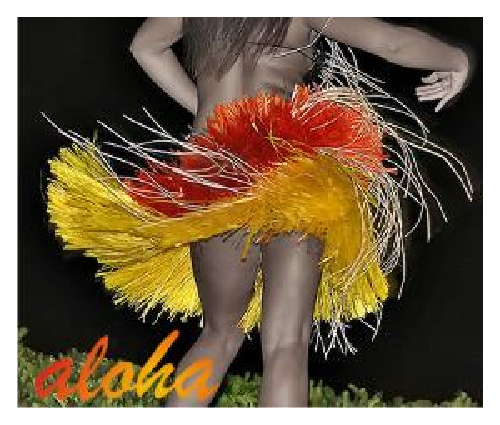
\includegraphics[width=70mm]{images/aloha-splash.eps}
          \vskip 20pt
          \huge \bfseries another linear optics helper application\par
     	  \vskip 20pt 
     	  \Large reference manual\par 
     	  \vskip 80pt
          \Large Kajetan Fuchsberger \par
        
        \end{flushleft}
        \vfill
        }}
    \null
  \end{titlepage}%
}


\newcommand {\mr}      {\mu rad}
\newcommand {\emity}   {\varepsilon_y}
\newcommand {\emitx}   {\varepsilon_x}
\newcommand {\dQ}      {\Delta_Q}
\newcommand {\Qh}      {Q_h}
\newcommand {\Qv}      {Q_v}
\newcommand {\Qu}      {Q_u}
\newcommand {\frev}    {f_{rev}}
\newcommand {\delp}    {\delta}
\newcommand {\Delp}    {\delta_p}
\newcommand {\qprh}    {\xi_h}
\newcommand {\qprv}    {\xi_v}
\newcommand {\qpru}    {\xi_u}
\newcommand {\qprhn}    {Q'_{h}}
\newcommand {\qprvn}    {Q'_{v}}
\newcommand {\qprun}    {Q'_{u}}
\newcommand {\xiind}    {\Delta \xi_{u}^{\mathrm{ind}}}
\newcommand {\xitrim}   {\Delta \xi_{u}^{\mathrm{Trim}}}
\newcommand {\ximeas}   {\xi_u^{\mathrm{meas}}}
\newcommand {\pdot}     {\dot{p}}
\newcommand {\ktwo}      {K_{2}}
\newcommand {\mmtwo}      {\mathrm{m}^{-2}}
\newcommand {\bthree}      {K_{2}L}
\newcommand {\bthreea}      {K_{2}^{a}L}
\newcommand {\bthreeb}      {K_{2}^{b}L}
\newcommand {\bthreen}      {b_{3}}
\newcommand {\bthreena}      {b_{3}^{a}}
\newcommand {\bthreenb}      {b_{3}^{b}}
\newcommand {\etal}   {{\it et al.}}
\newcommand {\murad}  {\mu \mathrm{rad}}

% newcommands KF
\newcommand{\titwo} {TI2}
\newcommand{\fitnorm}{\ensuremath{\Delta_\mathrm{rms}}}
\newcommand{\respmatmeas}{\ensuremath{R_{ij}^\mathrm{meas}}}
\newcommand{\respmatmodel}{\ensuremath{R_{ij}^\mathrm{model}}}
\newcommand{\noise}{\sigma}
\newcommand{\kick}{\delta}

\newcommand{\alohalong}{\emph{Aloha (another linear optics helper application)}}
\newcommand{\aloha}{\emph{Aloha}}

\begin{document}
\mytitlepage


\chapter{Introduction}
\label{sec:introduction}

\section{What is aloha}
\label{sec:whatiitis}

\alohalong{} was initiated during preparations for LHC comissioning and
startup. Its initial purpose was to serve as a tool for quick analysis of
kick-response data during the LHC comissioning phase in order to quickly
determine monitor- and corrector- gains as well as potential sources optics
errors. Later on it was extended to provide a wider range of tools for analysis
of accelerator optics.
For the time being it provides the following key features:
\begin{itemize}
  \item Fit algorithm: SVD
  \item Model-fits to kick-response and or dispersion data (seperately or in
  combination)
  \item Importer for Yasp files
  \item Full madx model integration. So it is possible to fit for
  a large variety of parameters in the madx model. (Not all at the moment, but
  number is increasing)
  \item easily extendable (e.g. importers, model)
\end{itemize}

\section{Structure of this document}
\label{sec:structure}
In \charef{principle} we will explain the mathematical principles used by
\aloha{}. In TODOREF we then wil focus more strongly on the implementation
details of \aloha{}.

\chapter{Analysis principle}
\label{cha:principle}

\section{Introducion}
\label{sec:principle.introduction}

The principle used extensively in \aloha{} is well known for a long time and
was for example used by the LOCO software \cite{SAFRA}. It is described in
detail for example in \cite{JW-RESP-SPS}. Nevertheless, since \aloha{} not only
allows fitting to kick-response data, but also to dispersion data by extending
the matrices, we want to describe this in some detail and explain especially
the \aloha-specific issues. 


In order to make the analysis-procedure more comfortable and flexible this time the algorithm was rewritten in java including a simple gui and a slim madx-api to gain more flexibility in accessing model data and varying model parameters.

In order to estimate the quality of a fit we use the rms of the elements of the relative difference-matrix:
\begin{equation}
\label{eq:fitnorm}
	\fitnorm = \sqrt{\frac{1}{N_v - 1} \sum_{i, j} \frac{\respmatmeas - \respmatmodel}{\frac{\noise_i}{\kick_j}}}.
\end{equation}
$\noise_i$ is the noise for monitor $i$, $\kick_j$ is the kick of corrector $j$,
$N_v$ is the number of all valid elements of the response-matrix and the sum must only contain valid elements. So this value will usually be greater than one and will converge to one, when the model error is of the same magnitude than the noise. This would correspond to a perfect fit in our sence.


\begin{thebibliography}{10}

\bibitem{SAFRA} J. Safranek, Nucl. Instr. Meth. A388 (1997) 27.

\bibitem{JW-RESP-SPS} J. Wenninger, {\it Orbit Response Measurements at the SPS},
CERN-AB-2004-009.

\end{thebibliography}

\end{document}
